\chapter{Problem Statement}
\label{chap:problem}
This chapter discusses previous work on the one legged hopper at IIT Bombay and formulates the exact problem statement and the scope 
for this project.

% 1. sayyad
%     poincar`e map ... read his abstract
%     saboo...sanmukh
% 2. londhe
%     describe mechanism
% 3. simit
%     contributions
% 4. siraj
%     contributions
\section{Previous work}
\subsection{1-D Hopper}
Vitthal Londhe~\cite{londhe} developed a 1D hopper and demonstrated in place hopping capabilities. The design was aimed at minimizing
the energy losses and making the robot easy to assemble and disassemble.
\begin{wrapfigure}{r}{0.4\textwidth}
\centering
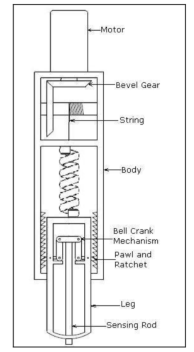
\includegraphics[scale =1.5]{fig/londhe.pdf}
\caption[Vertical Hopper]{Vertical Hopper \cite{londhe}}
\label{fig:2_londhe}
\end{wrapfigure}
Fig.~\ref{fig:2_londhe}, shows the major parts of this hopper viz. a winding motor with the energy pumping mechanism and a telescopic 
leg with a ratchet and paul constraint. The hopper is also confined to a fixed vertical axis. The leg is connected to a compression 
spring. A motor is used to compress this spring.\\

The constraint mechanism consists of a bell crank attached to the paul so that when the leg impacts upon the ground, the paul comes 
free of the ratchet teeth and the spring is free to compress further. This is the first use of impact forces for releasing the energy 
pumping mechanism in a one legged hopper. Thus the motor does not need to do work against the spring force to hold the leg in the compressed position. The latch mechanism mechanically latches the leg in place and unlatches it only when the leg touches the ground.
\subsection{SLOM Hopper}
Fig.~\ref{fig:2_hop2d} shows the prototype developed by Sharma and Gebretsadik~\cite{londhe} for which Vipul Saboo~\cite{saboo} 
designed and fabricated the EPM for it. He could also demonstrate hopping of the robot without active balancing.

The robot consists of a body and a telescopic leg of rectangular cross-section attached to the body by a spring. The leg also has a 
freely rotating ankle with a foot attached to it. The ankle ensures that the foot always falls flat on the ground irrespective of the 
orientation of the robot while touchdown.\\
\begin{figure}
\centering
\subfloat[SLOM hopper : sketch]{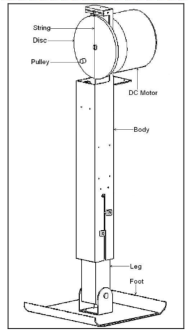
\includegraphics[scale = 1.5]{fig/saboo.pdf}\label{fig:2_hop2d}}
\hspace{1in}
\subfloat[Paul and ratchet]{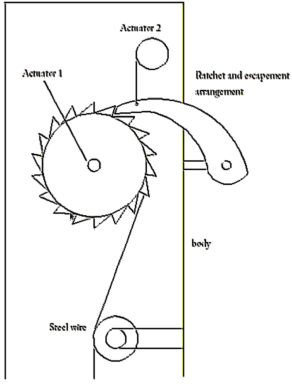
\includegraphics[scale = 1.2]{fig/ratchet.pdf}\label{fig:2_ratchet}}
\caption[2D SLOM hopper]{2D SLOM hopper \cite{saboo}}
\label{fig:2_saboo}
\end{figure}
To reduce the friction between the telescopic leg and the body, teflon bearings are used in sets of two on each of the four sides of 
the leg. The construction of the robot makes it very difficult to assemble and disassemble it. Also, the mass of the leg is almost 
${2/3}^{rd}$ of the mass of the body which results in huge energy loss of the system during impacts.
The EPM consists of a ratchet and a pawl with a voice-coil which activates the pawl. The voice-coil is electrically actuated by a 
mechanical limit switch attached on the foot of the robot. There is also a latch-type EPM where the motor can be switched off after 
the spring is compressed.\\

Simit \cite{simit} developed a treadmill and constraining mechanism (TCM) for the SLOM hopper. He also demonstrated an embedded system
for hopping height control using a feed-forward and PID controller. A ground station for gathering telemetry data from the TCM 
interface.

\subsection{Reaction wheel}
Siraj \cite{siraj} modeled attitude control of the hopper as a position control problem for the reaction wheel pendulum. He
demonstrated PID and LQR control strategies for the reaction wheel pendulum. Optimal control strategies have to be looked into because
as observed by Beuhler \cite{Bue_PassRun, ARLMono2}, almost 50\% of the total energy is utilized in swinging the leg mass i.e. in
attitude reorientation. A inertial measurement unit (IMU) using a complementary filter was also developed.

\section{Problem formulation}
The SLOM hopper was used as a test bed for devising hopping strategies by Saboo \cite{saboo}, Simit \cite{simit} and Siraj \cite{siraj}. However, it was an over-designed system with large energy losses due to impacts and friction. It was necessary to
remove these flaws in the robot before further work could be done on it. Hence, it was decided to go ahead with a completely new
mechanical design for the hopper keeping the following things in mind about the previous design.
\begin{enumerate}
\item
SLOM concept is quite novel and the new design will be based on it.
\item
Compression spring need an enclosure outside them to keep them in place when in compression. This results in frictional losses in
every cycle of energy pumping. Tension springs on the other hand do not have such frictional losses associated with them. It was thus
decided to use tension springs for the new design.
\item
The SLOM hopper could not hop above a height of 10 cm. The energy pumping mechanism (EPM) was the limiting factor. For achieving heights larger than this, we need to significantly reduce the leg mass and have a more energy efficient EPM.
\item
A reaction wheel should be present on the hopper and this will be used to reorient the robot to demonstrate both in-place hopping
and running capabilities.
\item
An embedded system along with on-board power supply shall be used to control the actuation, sensors and execute the control law.
\end{enumerate}


